\documentclass{beamer}
\usetheme{metropolis}

\usepackage[utf8]{inputenc}
\usepackage[portuguese]{babel}

\usepackage{color}
\usepackage{dirtytalk}
\usepackage{graphicx}
\usepackage{minted}
\usepackage{menukeys}
\usepackage{tabularx}

\graphicspath{{img/}}

\title{Minicurso de Java}
\subtitle{Introdução a Java}
\author{João Paulo Taylor Ienczak Zanette}

\newcommand{\icon}[1]{\raisebox{-.2\height}{\includegraphics[keepaspectratio,width=1em]{#1}}}

\begin{document}

\maketitle

\section{O que é programação?}

\section{Introdução a Java}
\subsection{Sobre a linguagem}

\begin{frame}{Princípios}
    \begin{enumerate}
        \item Deve ser "simples, orientada a objetos, e familiar";
        \item Deve ser "robusta e segura";
        \item Deve ser "de arquitetura neutra e portátil";
        \item Deve executar com "alta performance";
        \item Deve ser "interpretada, dinâmica e com suporte a threads ";
    \end{enumerate}
\end{frame}


\begin{frame}{Características gerais da linguagem}

    \begin{description}
        \item[Multiplataforma:] O mesmo código pode rodar em mais de uma plataforma
            sem a necessidade de recompilar;
        \item[Biblioteca padrão extensa:] Oferece diversos recursos já na
            biblioteca padrão, desde interfaces gráficas até manipulação de
            áudio/vídeo;
        \item[Alocação não-determinística:] Recursos alocados não são liberados
            explicitamente pelo programador, isso é feito por um
            \emph{Garbage-Collector};
        \item[Suporte a JIT:] Alguns trechos de código são otimizados em tempo de
            execução (\textit{Just In Time Compilation}).
    \end{description}

    \say{Java é uma mãezona: não deixa você fazer algo errado e ainda limpa
    tudo para você.}

\end{frame}


\begin{frame}{Onde é utilizada}
    \begin{itemize}
        \item Aplicações Desktop no geral (com ou sem interface gráfica);
        \item Comunicação com Banco de Dados em servidores de aplicações Web
            (\textit{back-end});
        \item Aplicações para dispositivos móveis Android;
        \item Sistemas embarcados e de tempo-real.
    \end{itemize}

    Foi bastante utilizada também para aplicações de celulares antigos (JavaME).
\end{frame}


\begin{frame}{A \textit{Java Virtual Machine}}
    Toda aplicação Java roda na JVM a partir de uma sequência de instruções
    geradas de um código Java. Essas instruções se chamam
    \textbf{\textit{Bytecode}}.
\end{frame}


\subsection{Criando uma aplicação}

\begin{frame}{Desenvolvendo uma aplicação Java simples}
    \begin{enumerate}
        \item Crie um arquivo de código Java (.java);
        \item Escreva o código (ver exemplo adiante), definindo o procedimento
            \texttt{main};
        \item Gere o \textit{Bytecode} da aplicação, que será lido pela JVM.
            Isso é feito pelo processo de \emph{Compilação};
        \item Execute o código chamando a JVM e indicando qual classe deve ser
            carregada. A JVM vai procurar e executar o procedimento
            \texttt{main} dessa classe.
    \end{enumerate}
\end{frame}


\begin{frame}[fragile]{Exemplo de código Java}
    \begin{minted}{java}
public class Application {
    public static void main(String... args) {
        System.out.println("Hello, World!");
    }
}
    \end{minted}

    \emph{OBS}: Toda aplicação Java inicia pelo \texttt{main}.
\end{frame}


\begin{frame}{Utilizando o compilador de Java}
    \begin{itemize}
        \item[] \icon{eclipse} Eclipse: \menu{Project > Build Project}.
            Executar a aplicação também chama o compilador.
        \item[] \icon{terminal} Terminal: \texttt{javac Application.java}
    \end{itemize}
\end{frame}


\begin{frame}{Processo de compilação de Java}
    \begin{center}
        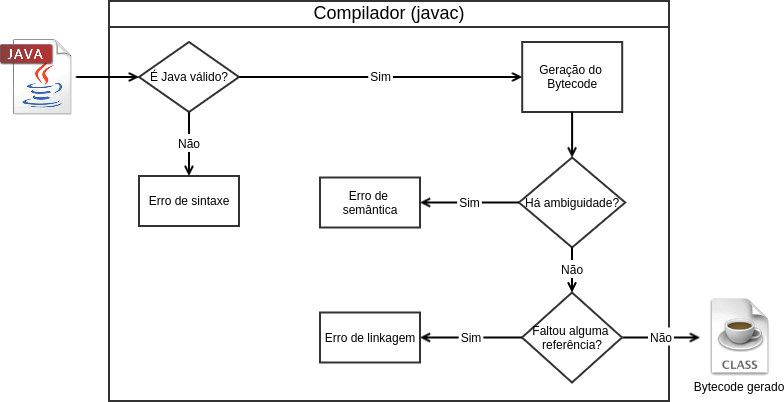
\includegraphics[keepaspectratio,width=1\textwidth,height=1\textheight]{compilation_scheme}
    \end{center}
\end{frame}


\begin{frame}[fragile]{\textit{Bytecode} gerado}
    \begin{minted}{java}
public class Application {
  public Application();
    Code:
       0: aload_0
       1: invokespecial #1 // java/lang/Object."<init>"
       4: return

  public static void main(java.lang.String...);
    Code:
       0: getstatic     #2 // java/lang/System.out
       3: ldc           #3 // Hello, World!
       5: invokevirtual #4 // java/io/PrintStream.println
       8: return
}
    \end{minted}
\end{frame}


\subsection{Execução de uma aplicação}

\begin{frame}{Executando uma aplicação Java}
    \begin{itemize}
        \item[] \icon{eclipse} Eclipse: Pressionar \keys{Ctrl+F11}
            (\menu{\icon{eclipse_run} Run}).

        \item[] \icon{terminal} Terminal: \texttt{java Application}
    \end{itemize}
\end{frame}


\begin{frame}{Execução do \textit{Bytecode} Java}
    \begin{center}
        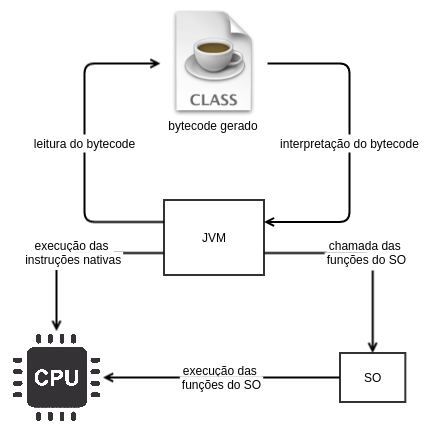
\includegraphics[keepaspectratio,width=1\textwidth,height=0.8\textheight]{jvm_scheme}
    \end{center}
\end{frame}

\begin{frame}[fragile]{Execução do \textit{Bytecode} Java}
    \begin{center}
        \emph{Importante:} A execução do código é sequencial, na ordem em que o
        código foi escrito. Portanto o seguinte de trecho de código:

        \begin{minted}{java}
            System.out.println("Linha 1");
            System.out.println("Linha 2");
            System.out.println("Linha 3");
            System.out.println("Linha 4");
        \end{minted}

        Produzirá a saída:

        \begin{minted}{bash}
            Linha 1
            Linha 2
            Linha 3
            Linha 4
        \end{minted}
    \end{center}
\end{frame}


\section{Trabalhando com programação}

\subsection{Variáveis}
\begin{frame}{Problema: Como guardar valores?}
    Não queremos fazer programas que apenas mostrem textos na tela. Porém, se
    quisermos programas mais complexos, precisamos de mais recursos.
    Para fazer uma loja, por exemplo, precisamos:

    \begin{itemize}
        \item Guardar as informações dos produtos (nomes, preços, etc.);
        \item Guardar a lista de compras do cliente;
        \item Calcular o total da compra para que o cliente possa pagar.
    \end{itemize}
\end{frame}

\begin{frame}{Solução: Variáveis}
    Variáveis são valores guardados na memória (geralmente RAM). Toda variável
    possui:
    \begin{description}
        \item[Identificador:] Nome para referenciá-la no código. Deve ser único
            dentro de um mesmo escopo.
        \item[Tipo:] Define o tipo de dado que ela guarda.
    \end{description}

    Há também, em programação, o conceito de \emph{constantes}, que funcionam
    semelhante às variáveis, porém não podem ser alteradas.
\end{frame}


\begin{frame}[fragile]{Criando uma variável}
    Para criar uma variável, basta \emph{declarar} ela, ou seja, escrever:

    \begin{minted}{java}
        Tipo nome;
    \end{minted}

    É possível ainda criar uma variável e já atribuir um valor a ela, da forma:

    \begin{minted}{java}
        Tipo nome = valor;
    \end{minted}
\end{frame}

\subsection{Tipos de dados}
\begin{frame}{Classificação de tipos}
    Os tipos de dados que podem ser guardados são divididos em:

    \begin{description}
        \item[Tipos Primitivos:] Valores indivisíveis, geralmente números;
        \item[Tipos Definidos por Usuário:] Tipos personalizados, compostos por
            diferentes valores internos.
    \end{description}
\end{frame}

\begin{frame}{Tipos primitivos}
    Numéros inteiros:
    \begin{center}
        \begin{tabular}{|l|l|l|}
            \hline Tipo           & Tamanho & Intervalo \\
            \hline \texttt{byte}  & 1 Byte  & $-128$ a $127$ \\
            \hline \texttt{short} & 2 Bytes & $-2^{15}$ a $2^{15}-1$ \\
            \hline \texttt{int}   & 4 Bytes & $-2^{31}$ a $2^{31}-1$ \\
            \hline \texttt{long}  & 8 Bytes & $-2^{63}$ a $2^{63}-1$ \\
            \hline
        \end{tabular}
    \end{center}

    Numéros reais:
    \begin{center}
        \begin{tabular}{|l|l|l|}
            \hline Tipo            & Tamanho & Intervalo \\
            \hline \texttt{float}  & 4 Bytes & $2^{-149}$ a $(2-2^{-23}) \cdot 2^{127}$ \\
            \hline \texttt{double} & 8 Bytes & $2^{-1074}$ a $(2-2^{-52}) \cdot 2^{1023}$ \\
            \hline
        \end{tabular}
    \end{center}

    Para caracteres há o tipo \texttt{char} (2 Bytes).
\end{frame}

\begin{frame}[fragile]{Operações: Soma}
    \begin{minted}{java}
        int a = 5;
        int b = 7;
        int sum = a + b;
    \end{minted}

    Após executar o trecho acima, o valor de \texttt{sum} será $12$.
\end{frame}

\begin{frame}[fragile]{Operações: Subtração}
    \begin{minted}{java}
        int a = 5;
        int b = 7;
        int sub = a - b;
    \end{minted}

    Após executar o trecho acima, o valor de \texttt{sub} será $-2$.
\end{frame}

\begin{frame}[fragile]{Operações: Multiplicação}
    \begin{minted}{java}
        int a = 5;
        int b = 7;
        int mul = a * b;
    \end{minted}

    Após executar o trecho acima, o valor de \texttt{mul} será $35$.
\end{frame}

\begin{frame}[fragile]{Operações: Divisão}
    \begin{minted}{java}
        int a = 5;
        int b = 7;
        int div = a / b;
    \end{minted}

    Esse é um caso especial em que, após executar o trecho acima, o valor de
    \texttt{div} será $0$. Isso se dá porque estamos utilizando números
    \emph{inteiros}. Se quisermos um resultado em números reais, precisamos utilizar variáveis
\end{frame}

\end{document}
